\section{Conception et architecture}
\subsection{Importance de la conception} La phase de conception d'un
logiciel est la plus critique de tout projet. En effet, negliger
(voir sauter) cette partie peut ammener à developper le logiciel sur
une base bancale peu ou pas adaptée, difficile à maintenir et à faire évoluer.

Nous avons donc voulu soigner cette partie avant de commencer à
programmer le jeu. Pour cela, nous avons choisi un mélange entre
méthode descendante et ascendante: la méthode déscendante étant
utilisée pour la partie structurante du programme, la méthode
ascendante pour les modules précis.

\subsection{Une conception modulaire}
\subsubsection{Idee principale} L'idée principale qui a guidé la
conception du squelette du programme est que le programme peut être vu
comme une machine à état. En effet, à chaque instant, le joueur vera
un aspect particulier du jeu (un état) tel que le menu principal ou
les options et c'est cet état du jeu qui influe sur la manière de traiter les événements,
d'afficher les informations à l'écran.

\subsubsection{Réalisation}
Afin de mettre en oeuvre cette idée, nous avons imaginé une structure
\textbf{game\textunderscore state} represantant un état de jeu courant. Cet
état de jeu peut être en autre caractérisé par: 
\begin{itemize}
  \item sa manière de gérer les évenements 
  \item sa fonction d'affichage : 
  \item son fond d'écran : \textit{surface SDL}
  \item des ressources spécifiques à l'état courant : 
  \item des ressources partagées entre les différents états :
    common\textunderscore data, défini après
\end{itemize}
 
Chaque état particulier du jeu ne sera alors qu'une instanciation du
modèle générique \textbf{game\textunderscore state} avec quelques spécialisations.

Comme nous le verrons, d'autres nécéssaire à la programmation s'ajouterons dans lors de la réalisation du code.
~\\

Les ressources partagées sont dans la structure
\textbf{game\textunderscore data}. Elle contient en particulier
\begin{itemize}
  \item le nom du joueur, demandé lors de la phase d'acceuil : \textit{string}
    (défini après)
  \item les options du jeu : (défini après)
  \item son score : \textit{entier}
\end{itemize}

~\\
Pour representer le jeu en lui même, nous avons pensé à une structure
\textbf{game} qui contient tous les états du jeu ainsi que la
propriété des données partagées entre état.

Pour centraliser le plus possible les appels relatifs à l'utilisation
de la SDL, nous avons choisi de créer une structure \textbf{displayer} qui
contient l'ensemble des données nécéssaires pour afficher quelque
chose à l'écran.

Au vu de la liste des objectifs que nous avons fait précédement, on
peut récapituler l'architecture de base comme il suit : 
~\\
\begin{center}
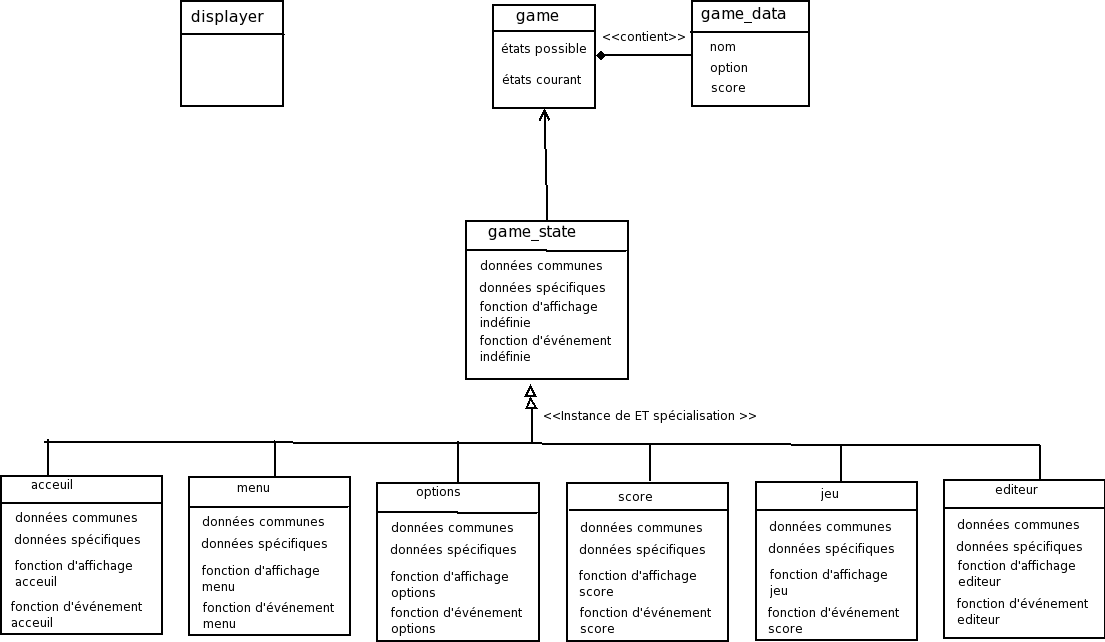
\includegraphics[scale=0.3]{img/principe.png}
\end{center}

On définit les transitions entre les états par le schéma suivant :
\begin{center}
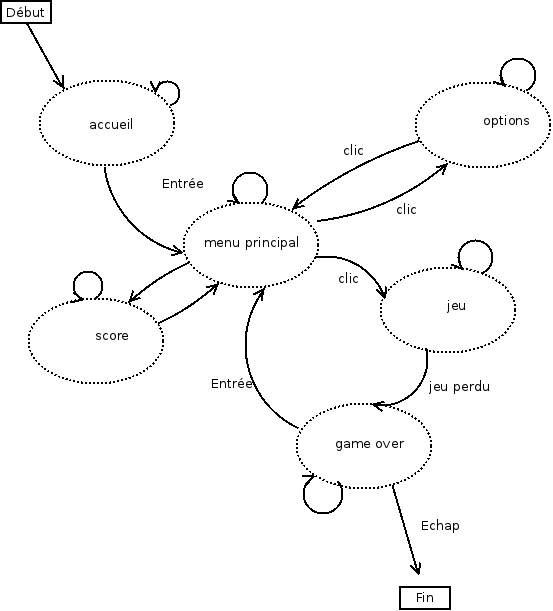
\includegraphics[scale=0.6]{img/transition.png}
\end{center}

\subsection{Les principaux TAD de base}
Lors de la conception, nous avons aussi trouvé un certain nombre de TAD qu'on peut qualifier de primitifs (dans le sens où il serront la brique de base d'autre TAD). On est ici clairement dans une conception ascendante.
~\\

Chaque TAD dont la copie n'est pas possible (tous sauf point et
sprite) doit fournir des fonctions de construction (build\textunderscore  xxx) ou
de création (create\textunderscore xxx) ainsi que de destruction.
Il existe une nuance entre la construction ou la création : la
création devra à la fois réserver un espace mémoire et l'initialiser
alors la construction ne devra assurer que l'initialisation.

\subsubsection{string}
Cette classe sert à représenter une chaîne de caractère. Elle a pour
but de simplifier au maximum la gestion des chaînes de
caractères. Elle doit offrir via son interface un certain nombre de
fonctionnalités dont celle pour la construction et destruction
(respectivement build\textunderscore  string et destruct\textunderscore string), accès à la taille
(size), à la capacité de la chaîne (capacity), ainsi que des fonctions
pour ajouter une chaîne à la fin (append\textunderscore string) et
retirer le dernier caractère de la chaîne (pop\textunderscore  string)

\subsubsection{point}
Simple agrégat de donné, il sert à représenter un point géométrique de
coordonnées x et y, il n'offre aucune interface particulière

\subsubsection{level}
Cette structure sert à représenter un niveau de jeu. Elle contient en autre : 
\begin{itemize}
  \item le nombre de point du niveau : entier
  \item l'ensemble des points du niveau : conteneur déterminé plus loin
  \item le nombre de balle avant le début du niveau : \textit{entier}
  \item le nombre de balle déjà insérée : \textit{entier}
  \item le nombre de différentes couleur qu'on peut utiliser (nombre
    fonction de la difficulté) : \textit{entier}
\end{itemize}

En plus des fonctions de création/destruction, le structure level
offre une fonction save\textunderscore level dont le rôle est de
sauvergarder un niveau dans un fichier donné.

\subsubsection{sprite}
Cette classe permet de representer une boule qui se situe dans le
cortege. Ses caractéristiques sont les suivantes : 
\begin{itemize}
  \item Le point courant où elle se situe : \textit{point}
  \item Une image pour representer la boule : \textit{surface SDL}
  \item le type de mouvement qu'elle est en train de suivre (avant,
    arrière ou sur place) : \textit{enumération}
  \item sa position dans le cortege : \textit{entier}
\end{itemize}

Un sprite offre comme principale interface une fonction pour mettre à
jour sa position (update\textunderscore position)

\subsubsection{projectile}
Cette structure permet de créer un projectile qui sera lancé sur le
cortège. Ses principales données sont : 
\begin{itemize}
  \item son image pour la representer : \textit{surface sdl}
  \item sa position actuelle : \textit{point}
  \item les composantes de sa vitesse en projection sur les axes x et
    y : \textit{nombres réels}
\end{itemize}

Un projectile donne comme interface : update\textunderscore projectile
pour mettre à jour la position du projectile ainsi que
create\textunderscore projectile pour créer un projectile.

\subsubsection{option}
Les options comme décrit dans la partie I comprennent : 
\begin{itemize}
  \item une variable sound pour indiquer si le son est actif ou non : \textit{entier}
  \item le numéro set graphique choisi : \textit{entier}
  \item le degré de difficulté choisi par le joueur : \textit{entier}
\end{itemize}

\subsection{Les principaux conteneurs}
La manière de stocker les différents éléments du jeu est un facteur
déterminant dans les performances du programme étant donné l'impact
qu'à (via de multiples allocations/désallocations inutiles) le choix
d'un contenur inapté à la situation.

\subsubsection{Conteneur pour les points dans un niveau}
Un chemin pour un niveau donné est décrit par un fichier dont la
première ligne donne le nombre de point dans le chemin. De plus, une
fois chargé, un niveau n'est pas amené à évoluer. Il paraît donc
logque d'utiliser un tableau pour gérer ces points.

\subsubsection{Conteneur pour les balles dans le cortège}
Au vu des modifications dans le cortège qui devront se produire
régulièrement, il paraissait assez logique d'utiliser une liste
chainée pour modéliser le cortège. Etant donné que nous aurions à
compter à partir d'un certain point de la liste, il est naturel de
choisir une liste doublement chainée.


